\chapter{Evaluation}
In this chapter, we evaluate the effectiveness of MADClean.
The evaluation focuses on the framework's ability to detect errors, the accuracy of its repair operations and its performance compared to relevant data cleaning approaches.
In addition, we analyze the impact of the individual framework modules through an ablation study.
\section{Experimental Setup}
To evaluate the performance of MADClean, we designed an experimental setup in which its results were compared against a set of baseline methods discussed in the literature review. 
These baselines were selected because they either use LLMs for data cleaning or demonstrate strong performance on benchmark datasets.
Several LLM-based cleaning methods discussed before could not be included in the evaluation because their source code is not publicly available (e.g., LLMClean, IterClean).
Other methods focus exclusively on specific error types, such as schema-level inconsistencies or DMVs (e.g., FAHES, SynODC). 
Since MADClean is designed for general-purpose data cleaning, these methods were excluded to ensure a meaningful comparison.

The evaluation is divided into two main phases:
\begin{enumerate}
  \item \textbf{Error Detection:} measuring whether the system correctly identifies erroneous cells in the dataset.
  \item \textbf{Error Correction:} measuring whether the system provides the correct values for the detected errors.
\end{enumerate}

In addition to accuracy metrics, we compare the runtime performance of all evaluated methods. 
For MADClean, we further conduct a more detailed analysis that includes an analysis of LLM token usage per dataset and an ablation study to evaluate the contribution of individual framework modules to the overall performance.
\newline\newline
Unless stated otherwise, all experiments involving LLM-based components use the \texttt{gemini-2.5-pro} model with default parameters (e.g., temperature = 1). 
Since LLMs are non-deterministic and therefore performance may vary between runs, results are reported as the mean of four independent executions to improve robustness. 
All experiments were conducted on a laptop equipped with an Intel(R) Core(TM) i7-8750H CPU (6 cores, 12 logical processors, base frequency 2.20 GHz), 16 GB of RAM, running Microsoft Windows 11 (Version 24H2).

\subsection{Datasets}
The evaluation is conducted using four benchmark datasets that are commonly used in prior data cleaning research. 
All datasets have a corresponding ground truth version, which is used as a reference for computing the evaluation metrics. 
Initially, these versions still contained inconsistencies and were manually curated to ensure a reliable evaluation. 
Examples are standardizing representations of missing values (e.g., replacing placeholders with NaN), converting formatting inconsistencies (e.g., converting '10\%' to 10) and fixing minor typos.
To evaluate the robustness of the cleaning methods, additional outliers were injected into the Movies and Beers datasets. 
The Rayyan dataset already contains natural outliers and was therefore not modified.
An overview of the datasets is provided below. 
Dataset size and error rates are reported separately in Table \ref{tab:datasets}.
\newline\newline
\textbf{Hospital} \cite{HOLOCLEAN} - A real-world, structured and redundant dataset describing hospitals and their attributes. 
The data consists primarily of short strings and numeric fields representing identifiers (e.g., zipcodes, phone numbers, IDs). 
Errors include typos caused by character replacement (e.g., replacing characters with 'x'), formatting inconsistencies (e.g., values stored with non-numeric characters instead of pure numerics), DMVs such as 'empty' and dependency violations.
\newline
\textbf{Beers} \cite{RAHA} - A real-world, structured and redundant dataset containing information about beers and their properties, such as alcohol by volume and brewery details. 
The dataset includes numeric columns, short strings and identifiers. 
Error types include missing values, formatting inconsistencies (e.g., '0.045\%' vs. 0.045, '12.0 oz' vs. '12.0 ounce'), dependency violations, schema violations where data from multiple columns is merged into a single column, and some outliers and typos.
\newline
\textbf{Movies} \cite{MDR} - A real-world, structured dataset containing information about movies, including cast, ratings, duration and textual descriptions. 
The dataset includes a diverse range of data types, such as dates, numeric values, identifiers, multi-value columns and free-text fields. 
Error types include missing values, DMVs (e.g., 'No description'), outliers and formatting inconsistencies, such as pattern violations, incorrect data types and duplicated values.
\newline
\textbf{Rayyan} \cite{RAYYAN} - A real-world dataset with a high degree of unstructured columns with heterogeneous representations and limited redundancy, describing academic journals and their metadata, including publication dates and authors. 
The dataset contains dates, numeric values, identifiers and text fields with inconsistent casing, diverse textual styles and substantial noise. 
Error types include typos, missing values, DMVs (e.g., -1, {NULL}), outliers and formatting inconsistencies

\begin{table}[h]
\centering
\resizebox{0.4\textwidth}{!}{
  \begin{tabular}{l|c|c}
  \toprule[1pt]
  \textbf{Dataset}  & \textbf{Size} & \textbf{Error rate} \\
  \midrule[1pt]
  Hospital & 1000 x 18 & 0.19 \\
  Beers & 2410 x 10 & 0.14  \\
  Movies & 7390 x 17 & 0.11  \\
  Rayyan & 1000 x 11 & 0.06  \\
  \bottomrule[1pt]
  \end{tabular}
}
\caption{Summary of dataset characteristics.}
\label{tab:datasets}
\end{table}

\subsection{Baselines}
To compare MADClean against existing methods, we include several data cleaning systems. 
All baselines support general-purpose data cleaning, except for SAGED, which is limited to error detection. 
For each method, the default parameters provided in the corresponding GitHub repositories were used to ensure fair comparisons. 
More detailed descriptions of these methods can be found in the related work section.
\newline\newline
\textbf{Raha}+\textbf{Baran} \cite{RAHA,BARAN} - An end-to-end data cleaning pipeline in which Raha performs error detection and Baran handles error correction based on the data from Raha. 
The error detection results therefore relate to Raha, while the error correction results depend on both Raha and Baran. 
Both components rely on machine learning models.
\newline
\textbf{HoloClean} \cite{HOLOCLEAN} - A probabilistic data cleaning system that detects and corrects errors by using integrity constraints and redundancy in the data. 
It is particularly effective on datasets where errors can be accurately modeled using constraints.
\newline
\textbf{RetClean} \cite{RETCLEAN} - An LLM-based data cleaning system that augments the cleaning process with contextual information from a data lake. 
In this evaluation, no external data lake is provided, so the model must rely on its own general knowledge and the context of other columns in the row for cleaning the values.
For RetClean, we implemented an asynchronous wrapper to reduce runtime and used the model \texttt{gemini-2.5.flash-lite}, as the estimated runtime with other models was impractically large.
Since Retclean's LLM is used only to analyze individual row contexts and generate cleaned values, rather than to perform complex tasks such as code generation, we consider this model choice to be a fair approximation.
\newline
\textbf{Cocoon} \cite{COCOON} - An LLM-based data cleaning approach that applies statistical analysis to summarize dataset characteristics and then uses these summaries to guide the LLM during the cleaning process.
\newline
\textbf{SAGED} \cite{SAGED} - A machine learning-based error detection system. Since SAGED requires labeled data for training, its base models were trained on the Flights \cite{HOLOCLEAN} dataset. Training on alternative datasets may affect performance.

\subsection{Evaluation Measures}
To evaluate the effectiveness of the data cleaning systems, we follow the standard evaluation protocol used in prior data cleaning research. 
The evaluation is performed at the cell level, where each cell in the dataset is treated as an individual decision outcome. 
We distinguish between error detection and error correction, while using a single, consistent definition of precision, recall and F1 score for both tasks.
\newline\newline
The term mask is commonly used in data cleaning literature to denote a boolean matrix that indicates specific properties of cells (e.g., whether a cell is erroneous, modified or correctly repaired). 
We therefore use this terminology throughout the evaluation.
\newline\newline
Let $D_d$ denote the dirty dataset and $D_{gt}$ the corresponding ground truth dataset. 
By comparing these two datasets, we construct the \emph{error mask}, which indicates the cells that are erroneous in the dirty dataset:
\[
E_{ij} =
\begin{cases}
1 & \text{if } D_d[i,j] \neq D_{gt}[i,j], \\
0 & \text{otherwise}.
\end{cases}
\]

Next, the data cleaning system is applied to $D_d$, producing the cleaned dataset $D_c$. 
From this, we define the \emph{change mask}, which captures all cells that were modified by the cleaning system:
\[
C_{ij} =
\begin{cases}
1 & \text{if } D_d[i,j] \neq D_c[i,j], \\
0 & \text{otherwise}.
\end{cases}
\]

Finally, we define a \emph{correction mask} that indicates whether the cleaned value matches the ground truth value:
\[
Q_{ij} =
\begin{cases}
1 & \text{if } D_c[i,j] = D_{gt}[i,j], \\
0 & \text{otherwise}.
\end{cases}
\]

This mask is used exclusively for evaluating correction quality.

\subsubsection{Error Detection}
For error detection, a cell is considered predicted as error if the cleaning system modifies it ($C_{ij}=1$). 
A cell is actually erroneous if it differs from the ground truth ($E_{ij}=1$).
Based on these definitions, we define:
\[
\textbf{True Positives (TP)} = \{(i,j) \mid E_{ij} = 1 \land C_{ij} = 1\}
\]
\indent Erroneous cells that are correctly detected (i.e., changed by the system).

\[
\textbf{False Positives (FP)} = \{(i,j) \mid E_{ij} = 0 \land C_{ij} = 1\}
\]
\indent Clean cells that are incorrectly modified by the system.

\[
\textbf{False Negatives (FN)} = \{(i,j) \mid E_{ij} = 1 \land C_{ij} = 0\}
\]
\indent Erroneous cells that are not detected by the system.

True Negatives (clean cells that remain unchanged) do not provide useful information in this context and are therefore excluded.

Using these sets, precision, recall and F1 score are computed as:
\[
\textbf{Precision} = \frac{|\text{TP}|}{|\text{TP}| + |\text{FP}|}
\]

\[
\textbf{Recall} = \frac{|\text{TP}|}{|\text{TP}| + |\text{FN}|}
\]

\[
\textbf{F1 score} = 2 \cdot \frac{\text{Precision} \cdot \text{Recall}}{\text{Precision} + \text{Recall}}
\]

Precision measures how many of the detected cells are truly erroneous, while recall measures how many of the actual erroneous cells are detected by the system.
The F1 score reflects the system's ability to balance missed errors and false detections.

\subsubsection{Error Correction}
For error correction, we evaluate whether the system not only detects an error but also repairs it correctly. A cell is considered correctly repaired if it is erroneous, modified by the system, and equal to the ground truth ($Q_{ij}=1$) after cleaning.
We therefore redefine the cases as:
\[
\textbf{True Positives (TP)} = \{(i,j) \mid E_{ij} = 1 \land C_{ij} = 1 \land Q_{ij} = 1\}
\]
\indent Erroneous cells that are changed and repaired correctly.

\[
\textbf{False Positives (FP)} = \{(i,j) \mid C_{ij} = 1 \land Q_{ij} = 0\}
\]
\indent Cells that are modified but not repaired correctly, including both incorrectly changed clean cells and incorrectly repaired erroneous cells.

\[
\textbf{False Negatives (FN)} = \{(i,j) \mid E_{ij} = 1 \land Q_{ij} = 0\}
\]
\indent Erroneous cells that are not repaired correctly, either because they were not changed or because they were changed to an incorrect value.

We use the same formulas for precision, recall and F1-score as described above to maintain consistency. 
In this context, precision reflects how many of the modified cells are repaired correctly, while recall reflects how many of the true errors in the dataset are repaired correctly.

\section{Results}
In this section, we present the experimental results of . 
We first evaluate error detection and correction performance using the results reported in the tables and the analysis of the cleaned datasets. 
We discuss observed cleaning behavior and compare MADClean with baseline methods. 
Finally, we analyze runtime performance and provide a more in-depth evaluation of the framework.

\subsection{Error Detection Results}
The error detection results in Table \ref{tab:detection_results} show that MADClean consistently outperforms the baseline methods across most datasets, yielding near-perfect F1 scores for all datasets except Rayyan.
On Rayyan, Raha+Baran slightly outperforms the MADClean in terms of F1 score.
MADClean demonstrates high recall across all datasets, showing that it effectively identifies erroneous cells. 
At the same time, it maintains high precision, meaning that only few clean cells are incorrectly flagged. 
This is an important property for data cleaning systems, as unnecessary changes to clean values can negatively affect overall data quality.
\newline\newline
Among the baseline methods, HoloClean exhibits the weakest detection performance across datasets, largely due to its preprocessing step that converts all values to lowercase, which introduces many false positives. 
In addition, HoloClean failed to complete the cleaning process for the Movies dataset due to excessive memory requirements (it attempted to allocate 50 GB of memory). 
RetClean also shows low detection performance and did not finish execution on the Movies dataset within the 15-hour timeout. 
Analysis of its cleaned outputs indicates a high number of false positives, mainly caused by unstable LLM responses and inconsistent parsing (which may be partly attributable to the use of a different model and to unhandled output formats observed in the source code). 
SAGED achieves moderate detection performance but suffers from low precision, as it tends to overgeneralize errors and frequently flags entire columns as erroneous even when only a subset of cells contains errors. 
Cocoon performs reasonably well on the Hospital and Beers datasets but is less consistent on the Movies and Rayyan datasets, where detection accuracy drops notably. 
Finally, Raha+Baran shows strong and consistent detection performance across the datasets, achieving F1 scores above 0.90 on all datasets except Rayyan. 
Its performance is comparable to that of MADClean, highlighting that it remains a strong baseline for error detection tasks.

\begin{table}[h]
\centering
\resizebox{\textwidth}{!}{
  \begin{tabular}{l|ccc|ccc|ccc|ccc}
  \toprule[1.5pt]
  \textbf{Method}  & \multicolumn{3}{c|}{\textbf{Hospital}} & \multicolumn{3}{c|}{\textbf{Beers}} & \multicolumn{3}{c|}{\textbf{Movies}} & \multicolumn{3}{c}{\textbf{Rayyan}} \\
  \midrule[1pt]
    & \textbf{P} & \textbf{R} & \textbf{F1} & \textbf{P} & \textbf{R} & \textbf{F1} & \textbf{P} & \textbf{R} & \textbf{F1} & \textbf{P} & \textbf{R} & \textbf{F1} \\
  \midrule[1pt]
  Raha+Baran & \textbf{1.00} & 0.92 & 0.96 & \textbf{1.00} & 0.96 & 0.98 & 0.95 & 0.91 & 0.93 & \textbf{0.84} & 0.64 & \textbf{0.73} \\
  HoloClean & 0.95 & 0.12 & 0.22 & 0.04 & 0.17 & 0.07 & - & - & - & 0.09 & 0.73 & 0.16 \\
  RetClean & 0.31 & 0.30 & 0.31 & 0.40 & 0.68 & 0.50 & - & - & - & 0.08 & 0.69 & 0.14 \\
  Cocoon & 0.72 & 0.93 & 0.81 & 1.00 & 0.91 & 0.95 & 0.24 & \textbf{1.00} & 0.38 & 0.19 & 0.33 & 0.24 \\
  SAGED & 0.52 & 0.91 & 0.66 & 0.52 & 0.91 & 0.66 & 0.44 & 0.94 & 0.60 & 0.09 & 0.46 & 0.15 \\
  \midrule[1pt]
  MADClean & 0.98 & \textbf{0.99} & \textbf{0.99} & 0.99 & \textbf{0.99} & \textbf{0.99} & \textbf{0.97} & \textbf{1.00} & \textbf{0.99} & 0.65 & \textbf{0.81} & 0.67 \\
  \bottomrule[1.5pt]
  \end{tabular}
}
\caption{Detection results for MADClean and baselines across datasets.}
\label{tab:detection_results}
\end{table}

Detection performance is generally strongest on highly structured datasets, such as Hospital, Beers and Movies. 
In these settings, MADClean successfully identifies a wide range of errors across textual and numeric columns and relational fields. 
This success is largely due to the structured nature of these datasets, the presence of redundancy and the ability of the framework to leverage functional dependencies and column-level context. 
For example, datasets like Beers contain many columns with short, redundant strings or numeric values, which allows the LLM to infer dominant patterns and derive generalized detection rules effectively.
\newline\newline
Common textual errors are handled effectively, including typos, inconsistent whitespace and semantic inconsistencies. 
It reliably identifies ambiguous missing value placeholders such as 'empty', 'Add a plot', 'No description', -1 and 'NULL', which are often difficult to detect using rule-based methods.  
In addition, inconsistent use of abbreviations, such as 'Co.' when 'Company' is the dominant representation, is consistently flagged as erroneous. 
Similar behavior is observed for columns where values deviate from the dominant string pattern, such as city fields that inconsistently include state abbreviations (e.g., 'San Francisco CA'). 
Both syntactic and semantic errors are detected, particularly in named entities such as city or state names, where misspellings or incorrect entries (e.g., neighborhoods appearing in city columns) are identified. 
These cases highlight the advantage of LLM-based semantic reasoning, which several baseline methods, including Cocoon, do not fully capture.
\newline\newline
MADClean also performs well on formatting and pattern-based errors. 
In the Movies dataset, identifier columns that follow a regular expression pattern are handled effectively: deviations from the dominant pattern are consistently detected, while all baseline methods fail to identify these violations. 
Duplicate values, both numeric (e.g., '2005 2005') and textual (e.g., repeated names in multi-value fields), are also reliably detected. 
In addition, date entries that deviate from the dominant format (e.g.,  'Nov 24, 2011 USA' instead of '24 November 2011 (USA)') are flagged as errors, whereas the other baselines fail to detect these inconsistencies.
\newline\newline
Numeric formatting inconsistencies are detected with high accuracy. 
Columns containing values such as '12.0 oz', '12.0 ounce', '97\%' or '33 patients' are consistently flagged as erroneous due to the presence of non-numeric characters. 
While Cocoon and Raha+Baran also identify many of these issues, MADClean provides more complete detection overall. 
In addition, most outliers are detected, while all other baseline methods, except SAGED in some cases, largely fail to identify them.
\newline\newline
The framework is also effective at enforcing functional dependencies. 
The majority of violations are correctly identified and missing values that can be inferred using functional dependencies are flagged accordingly. 
In contrast, Cocoon and SAGED fail to detect most of the violations, HoloClean only identifies imputable missing values and Raha+Baran detects only a subset of the functional dependency pairs, missing many violations.
\newline\newline
Only a small number of misdetections are introduced. 
Some false negatives occur for highly irregular errors, such as random character replacements (e.g., arbitrary 'x' substitutions in Hospital). 
These errors lack a consistent pattern, making generalized detection difficult for both MADClean and Raha+Baran, which both rely on a limited subset of the dataset to infer rules that are applied globally. 
Furthermore, minor false positives occur primarily in string values, where special symbols such as trademark characters are flagged for removal.
\newline\newline
Performance declines substantially on unstructured datasets such as Rayyan, which contain heterogeneous column formats, ambiguous styles and limited redundancy. 
These characteristics make it difficult for the LLM to infer stable, column-wide detection rules. 
In particular, the lack of dominant patterns limits the LLM's ability to reliably distinguish between clean and erroneous values, leading to both missed errors and incorrect flagging of valid entries.
Moreover, the presence of many heterogeneous error types further complicates detection, as pattern-based reasoning is less effective when errors do not follow consistent, repeatable structures. 
For example, some text columns contain a mix of capitalized and lowercase entries without a consistent formatting pattern, preventing the LLM from learning a common structure and causing valid stylistic variations to be flagged as errors.
In contrast, datasets with more regular error patterns allow the generalization of detection rules more accurately, resulting in higher precision and recall.
Nevertheless, MADClean still matches or exceeds the overall performance of most baseline methods. 
Detection performance remains strongest in the more structured columns of this dataset, such as those containing language or ISSN entries, where dominant patterns can be identified. 
Recall remains relatively high in these cases, as many erroneous values are still correctly identified.
However, many clean values are also incorrectly flagged as errors, leading to lower precision. 
This limitation is shared by all baseline methods, with MADClean generally outperforming them, except for Raha+Baran.

\subsection{Error Correction Results}
The error correction results shown in Table \ref{tab:correction_results} further highlight the effectiveness of MADClean. 
It outperforms all baseline methods or achieves equivalent performance across all datasets, while maintaining high precision and recall on most datasets. 
For three of the four benchmark datasets, F1 scores above 0.96 are achieved. 
High precision indicates that most detected errors are repaired correctly, while high recall shows that the majority of all existing errors in the dataset are successfully corrected.
\newline\newline
In contrast, several baseline methods struggle with reliable error correction. 
RetClean exhibits low precision, indicating that many detected errors are repaired incorrectly. 
HoloClean achieves near-zero correction performance on most datasets, with the exception of Hospital. 
This can be explained by the high level of redundancy and the strong constraints in the dataset, which HoloClean can effectively utilize to repair values. 
Cocoon shows high recall on three datasets but has lower precision and exhibits inconsistent performance across datasets. 
Raha+Baran achieves strong correction results, with F1 scores above 0.91 on three of the four datasets, confirming its effectiveness as an end-to-end data cleaning system. 
Since SAGED is designed only for error detection, it is excluded from this evaluation.

\begin{table}[h]
\centering
\resizebox{\textwidth}{!}{
  \begin{tabular}{l|ccc|ccc|ccc|ccc}
  \toprule[1.5pt]
  \textbf{Method}  & \multicolumn{3}{c|}{\textbf{Hospital}} & \multicolumn{3}{c|}{\textbf{Beers}} & \multicolumn{3}{c|}{\textbf{Movies}} & \multicolumn{3}{c}{\textbf{Rayyan}} \\
  \midrule[1pt]
    & \textbf{P} & \textbf{R} & \textbf{F1} & \textbf{P} & \textbf{R} & \textbf{F1} & \textbf{P} & \textbf{R} & \textbf{F1} & \textbf{P} & \textbf{R} & \textbf{F1} \\
  \midrule[1pt]
  Raha+Baran & \textbf{1.00} & 0.92 & \textbf{0.96} & 0.94 & 0.91 & 0.93 & 0.93 & 0.90 & 0.91 & \textbf{0.61} & 0.46 & 0.52 \\
  HoloClean & 0.95 & 0.12 & 0.22 & 0.00 & 0.00 & 0.00 & - & - & - & 0.00 & 0.04 & 0.01 \\
  RetClean & 0.05 & 0.04 & 0.04 & 0.29 & 0.50 & 0.37 & - & - & - & 0.02 & 0.20 & 0.04 \\
  Cocoon & 0.71 & 0.91 & 0.79 & \textbf{1.00} & 0.91 & 0.95 & 0.23 & 0.95 & 0.37 & 0.18 & 0.31 & 0.23 \\
  \midrule[1pt]
  MADClean & 0.96 & \textbf{0.97} & \textbf{0.96} & 0.99 & \textbf{0.99} & \textbf{0.99} & \textbf{0.97} & \textbf{1.00} & \textbf{0.98} & 0.59 & \textbf{0.75} & \textbf{0.61} \\
  \bottomrule[1.5pt]
  \end{tabular}
}
\caption{Correction results for MADClean and baselines across datasets.}
\label{tab:correction_results}
\end{table}

Textual error correction is one of the framework's strongest components. 
It introduces few miscorrections and follows dominant dataset formats using column-level context, as it is designed to minimize stylistic changes and ensure consistency within each column. 
Other LLM-based baseline methods such as Cocoon and RetClean often introduce unnecessary modifications, such as rewriting full addresses or inconsistently modifying capitalization. 
In contrast, MADClean preserves valid representations while correcting true inconsistencies. 
Misspellings, inconsistent abbreviations or incorrect semantic entries are standardized or normalized to the correct values in most cases. 
These corrections leverage the LLM's semantic understanding, which is largely absent in non-LLM-based baseline methods.
\newline\newline
Formatting inconsistencies in textual columns are corrected using column-level patterns or functional dependencies where possible, and otherwise set to NaN. 
This ensures a single, consistent representation within each column. 
Date values are standardized to the dominant format observed in the column, avoiding the many false positives introduced by baselines such as Cocoon, which convert date entries into alternative datetime formats.
For example, in the Release Date column of the Movies dataset, which follows the dominant format '3 June 1988 (USA)', alternative representations such as 'May 10, 1973 France' are standardized to '10 May 1973 (France)'. 
Similarly, in the Language column of the Rayyan dataset, variants such as 'eng', 'English' and 'ENG' are normalized to a single consistent representation.
\newline\newline
The framework performs particularly well on numeric columns. 
Formatting inconsistencies such as percentages, units or mixed textual representations (e.g., '55 min' and '1 hr. 23 min.') are removed, converting values into pure numeric types. 
These conversions improve consistency and downstream usability for analytical and machine learning tasks. 
While Cocoon applies similar transformations in some cases, it does so inconsistently across columns and datasets.
Other baselines either ignore these inconsistencies or apply partial, inconsistent corrections, leaving noisy non-numeric values in the data. 
MADClean is the only method that applies these corrections consistently across all numeric columns. 
For example, in the Beers dataset, the ounces column contains various formats such as '12.0 oz', '12.0 oz.', '12.0 ounce' and '12.0 OZ.', all of which are converted to the pure numeric value 12.0. 
Likewise, in the Movies dataset, mixed duration formats including '85 min', '140 min' and '1 hr. 39 min.' are standardized to numeric minute values.
\newline\newline
Outliers are handled effectively by the framework. 
It distinguishes between true outliers, placeholder values and legitimate extreme values. 
True outliers are usually corrected by replacing them with the median, while placeholder values indicating missing data are converted to NaN. 
For example, in the ibu column of the Beers dataset, extreme values such as 2500 are treated as true outliers and replaced with the median, whereas placeholder values such as 9999 are interpreted as missing value placeholders and converted to NaN.
In some cases, when uncertainty is high, values are conservatively set to NaN rather than applying an incorrect repair.
\newline\newline
Functional dependency reasoning further enhances correction quality. 
Errors that cannot be corrected from cell-level context alone are repaired using functional dependency information. 
Invalid identifier values (e.g., '100x8' instead of '10018') are corrected based on redundancy in related columns, and missing values are imputed when dependencies allow reliable inference. 
A notable example illustrating the effectiveness of using an LLM as a semantic decision-maker involves the functional dependency between columns brewery\_name and brewery\_id. 
Multiple rows corresponding to 'Oskar Blues Brewery' have different IDs and cities because the brewery operates in multiple locations. 
This triggers a statistical dependency violation, and a naive repair strategy based on majority voting would incorrectly overwrite these valid differences (i.e., standardizing all rows to a single ID). 
In contrast, MADClean uses the row-level context to infer the true logic and preserves the legitimate variations, thereby maintaining semantic correctness rather than enforcing purely statistical consistency.
\newline\newline
Rare incorrect repairs occur when the LLM replaces a detected error with NaN instead of inferring the correct value, usually due to insufficient context. 
Most false positives are minor formatting changes, such as inserting spaces after commas or converting curly apostrophes to straight ones. 
Although these changes are counted as errors in evaluation, they improve readability and consistency and could be avoided by stricter validation. 
This behavior demonstrates that LLMs may apply learned formatting habits even when explicitly instructed not to, reinforcing the importance of validation mechanisms within the framework.
\newline\newline
Error correction performance is weakest in unstructured free-text columns, such as those in the Rayyan dataset. 
Similar to the detection setting, the absence of consistent patterns and clear formatting structures limits the LLM's ability to infer how clean values should look like.
Complex columns containing HTML entities, corrupted symbols or inconsistent formatting further reduce the ability to infer reliable repair strategies. 
In these cases, detected errors are often replaced with NaN rather than corrected, as no reliable correction can be inferred. 
This limitation reflects the inherent difficulty of cleaning unstructured text and is shared by all baseline methods.

\subsection{Runtime and Token Usage}
The runtime results in Table \ref{tab:runtimes} indicate that MADClean outperforms Raha+Baran and RetClean and achieves a runtime comparable to Cocoon. 
HoloClean is faster but its cleaning performance is substantially lower. 
While Raha+Baran achieves similar cleaning quality, it requires significantly more time, highlighting that MADClean is the more efficient choice for practical data cleaning.
Interestingly, the Movies dataset, which is the largest in terms of rows, exhibits the shortest runtime among all datasets for MADClean. 
This is because the it samples datasets and generates cleaning code rather than directly operation on all cells, making runtime largely independent of the total number of rows. 
Instead, runtime primarily scales with the number of columns and the number of detected functional dependencies. 
For example, the Hospital dataset has many columns and functional dependencies, resulting in the longest runtime.
The Rayyan dataset also exhibits a relatively high runtime. 
As described earlier, difficulties in inferring consistent cleaning rules likely cause many operations to be rejected by the Validation Agent, requiring multiple retries and increasing overall runtime.

\begin{table}[h]
\centering
\resizebox{0.6\textwidth}{!}{
  \begin{tabular}{l|c|c|c|c}
  \toprule[1pt]
  \textbf{Method}  & \textbf{Hospital} & \textbf{Beers} & \textbf{Movies} & \textbf{Rayyan} \\
  \midrule[1pt]
  Raha+Baran & 17051 & 9163 & 48368 & 9439 \\
  HoloClean & 225 & 158 & - & 192 \\
  RetClean & 8462 & 13506 & - & 5271 \\
  Cocoon & 763 & 148 & 585 & 426 \\
  \midrule[1pt]
  MADClean & 632 & 303 & 171 & 556 \\
  \bottomrule[1pt]
  \end{tabular}
}
\caption{Runtime (s) for MADClean and baselines across datasets.}
\label{tab:runtimes}
\end{table}

A similar pattern is observed in token usage (see Table \ref{tab:token_usage}). 
The Hospital dataset consumes many tokens due to its large number of columns and existing dependencies, while Rayyan consumes many tokens because of the complexity and heterogeneity of its data. 
Although the Movies dataset is processed faster than Beers, it requires more tokens. 
This is because Movies contains long string values, which increase token usage, while Beers consists mainly of short strings and numeric values, which are less costly to process. 
The input token size for Movies is nearly twice that of Beers, explaining the higher total token count despite the shorter runtime.

\begin{table}[h]
\centering
\resizebox{0.5\textwidth}{!}{
  \begin{tabular}{l|c|c|c}
  \toprule[1pt]
  \textbf{Dataset} & \textbf{Input} & \textbf{Output} & \textbf{Total} \\
  \midrule[1pt]
  Hospital & 366,907 & 231,973 & 598,880 \\
  Beers & 127,876 & 69,876 & 197,752 \\
  Movies & 239,393 & 90,325 & 329,718 \\
  Rayyan & 306,225 & 194,494 & 500,722 \\
  \bottomrule[1pt]
  \end{tabular}
}
\caption{Token usage of MADClean across datasets.}
\label{tab:token_usage}
\end{table}


\subsection{Ablation Study}
To evaluate the contribution of the different modules of MADClean, we conducted an ablation study, comparing the full framework with three variants: one without the functional dependency detection tool, one without the Validation Agent and one using a basic prompt instead of a detailed, type-specific prompt. 
By analyzing changes in detection and correction performance across these variants, we can assess the relative importance of each module. 
For consistency, all results are averaged over two independent runs. The results are presented in Figures \ref{fig:ablation_study_det} and \ref{fig:ablation_study_cor}.

\begin{figure}[H]
    \centering
    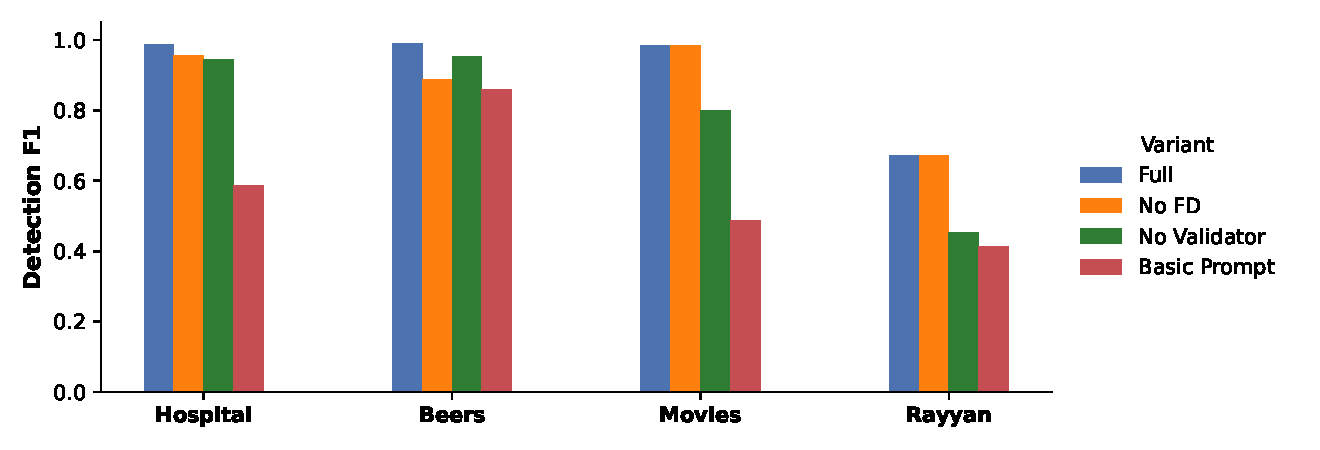
\includegraphics[width=0.8\textwidth]{Figures/ablation_detection.pdf}
    \caption{Ablation study results for detection F1 scores across datasets.}
    \label{fig:ablation_study_det}
\end{figure}

\begin{figure}[H]
    \centering
    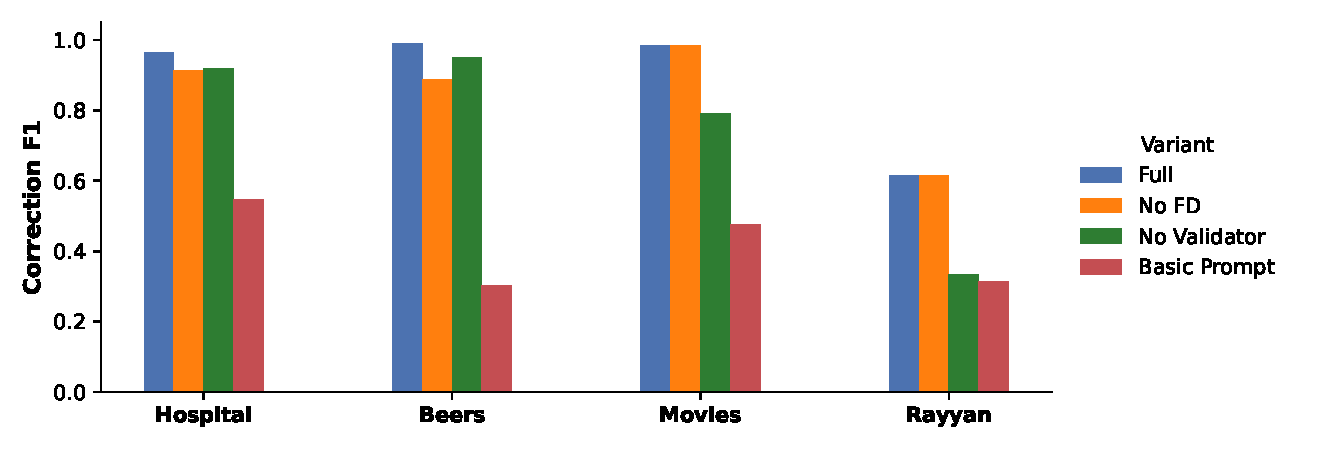
\includegraphics[width=0.8\textwidth]{Figures/ablation_correction.pdf}
    \caption{Ablation study results for correction F1 scores across datasets.}
    \label{fig:ablation_study_cor}
\end{figure}

Removing the functional dependency detection tool primarily affects the Hospital and Beers datasets, as they are the only datasets in the benchmark that contain functional dependencies. 
The results for the other datasets remain unchanged.
For the Hospital dataset, the impact is relatively small: F1 score for detection decreases from 0.99 to 0.96 and for correction from 0.96 to 0.91. 
Most functional dependency violations in this dataset correspond to simple typos, and the LLM can often infer the correct values using column-level redundancy, which minimizes the effect of removing the tool. 
The performance drop on the Beers dataset is more noticeable, with F1 score for both detection and correction falling from 0.99 to 0.89. 
In this setting, missing values in the state column are no longer imputed and violations in the city column remain uncorrected, although most other cells are still cleaned correctly. 
As shown in Table \ref{tab:ablation_study}, skipping the dependency detection tool slightly reduces runtime, as fewer LLM API calls are required, while token usage is largely unaffected. 
Overall, these results indicate that functional dependency reasoning is particularly valuable for correcting missing values and violations that cannot be resolved using column-level context alone.
\newline\newline
Removing the Validation Agent has a more substantial effect on overall performance. 
For the structured and redundant Beers and Hospital datasets, the F1 score drops modestly, approximately five percentage points, as the LLM can still infer correct cleaning operations based on the consistent formatting patterns in these datasets. 
Most formatting inconsistencies are repaired correctly and the few false positives are primarily due to minor deviations from the dominant format, such as changes in capitalization or abbreviation expansion, which the Validation Agent would normally prevent. 
In contrast, the impact is significantly larger for for the Movies and Rayyan datasets.
For Movies, the F1 score drops by 19 percentage points, and for Rayyan by 24 points. 
The Movies dataset contains multiple valid cleaning alternatives, while Rayyan is more heterogeneous and contains many ambiguous entries. 
Without the Validation Agent, the LLM applies a broader range of incorrect modifications, such as changing date formats, altering the structure of multi-value columns (e.g., inserting spaces after delimiters in comma-sperated values) or changing capitalization, leading to a significant increase in false positives. 
This again illustrates that, even when explicitly instructed not to perform such changes, the LLM may revert to learned formatting conventions from its training data and apply corrections that are not supported by common patterns in the dataset.
The removal of the Validation Agent also affects runtime and token usage.
Both of which are slightly reduced, as fewer retires are required when cleaning operations are accepted on the first attempt.
However, this reduction comes at the cost of substantially lower precision, highlighting the Validation Agent's critical role in maintaining precision, especially in datasets with complex or variable formatting.
\newline\newline
The variant using a basic prompt exhibits the largest performance decline. 
In this setting, the high-quality prompts for both the Recommender and Validation Agents are replaced with simplified prompts.
These prompts contains only generic instructions (e.g., to clean the data or enforce functional dependencies) and the same data sample as in the original prompt, but excludes all type-specific guidance and examples.
On the Beers dataset, detection F1 score remains relatively high at 0.86, but correction F1 score drops sharply to 0.30. 
For Hospital, both detection and correction F1 score decrease by approximately 40 percentage points. 
The Movies dataset experiences a decline of around 50 percentage points, and Rayyan drops by 28 percentage points. 
The primary cause of this drop is the incorrect modification of string values: capitalization is changed inconsistently, abbreviations are expanded and metadata is removed, resulting in numerous false positives. 
Formatting corrections are also incomplete.
For instance, numeric columns such as score, sample, ounces and abv are not consistently standardized to pure numeric columns. 
Multi-value columns are frequently reformatted incorrectly (e.g., strings converted to lists or with inserted spaces after commas), further reducing precision. 
These results highlight that detailed instructions and contextual examples are essential for guiding the LLM toward consistent and reliable cleaning behavior, and that removing this guidance leads to unstable transformations and a substantial increase in false positives.
Despite these challenges, basic error types such as typos, DMVs and pattern violations are still detected. 
Runtime is slightly longer for this variant, likely due to additional retries required for generated cleaning operations to satisfy the Validation Agent, while token usage remains similar.

\begin{table}[h]
\centering
\resizebox{\textwidth}{!}{
  \begin{tabular}{l|ccc|ccc|ccc|ccc}
  \toprule[1pt]
  \textbf{Ablation} & \multicolumn{3}{c|}{\textbf{Hospital}} & \multicolumn{3}{c|}{\textbf{Beers}} & \multicolumn{3}{c|}{\textbf{Movies}} & \multicolumn{3}{c}{\textbf{Rayyan}} \\
  \midrule[1pt]
    & \textbf{Runtime} & \textbf{Input} & \textbf{Output} & \textbf{Runtime} & \textbf{Input} & \textbf{Output} & \textbf{Runtime} & \textbf{Input} & \textbf{Output} & \textbf{Runtime} & \textbf{Input} & \textbf{Output} \\
  \midrule[1pt]
  Full & 632 & 366,907 & 231,973 & 303 & 127,876 & 69,876 & 171 & 239,393 & 90,325 & 556 & 306,225 & 194,494 \\
  No FD & 598 & 330,474 & 212,937 & 245 & 133,777 & 73,116 & 171 & 239,393 & 90,325 & 556 & 306,225 & 194,494 \\
  No Validator & 397 & 121,605 & 164,230 & 163 & 50,140 & 42,995 & 96 & 109,448 & 61,282 & 186 & 60,582 & 77,875 \\
  Basic Prompt & 636 & 352,567 & 304,201 & 351 & 88,730 & 82,582 & 334 & 257,075 & 145,766 & 718 & 383,384 & 274,720 \\
  \bottomrule[1pt]
  \end{tabular}
}
\caption{Runtime (s) and token usage across datasets.}
\label{tab:ablation_study}
\end{table}

Overall, the ablation study demonstrates that each module contributes meaningfully to the framework's performance, with prompt engineering having the largest impact, yielding an average difference of 47 percentage points in F1 score between the proposed prompts and a basic prompt.
High-quality, type-specific prompts provide explicit instructions and examples, ensuring that the LLM applies cleaning operations consistently and according to the dataset's structure, rather than relying on generalized heuristics from its training data. 
Functional dependency reasoning further improves correction quality by enabling context-aware corrections that leverage relationships between columns, particularly for missing values and values that cannot be repaired using column-level information.
The Validation Agent further supports overall reliability by preventing unwanted modifications, thereby preserving precision and improving robustness, especially in complex or heterogeneous datasets.
